\begin{minipage}{0.49\linewidth}
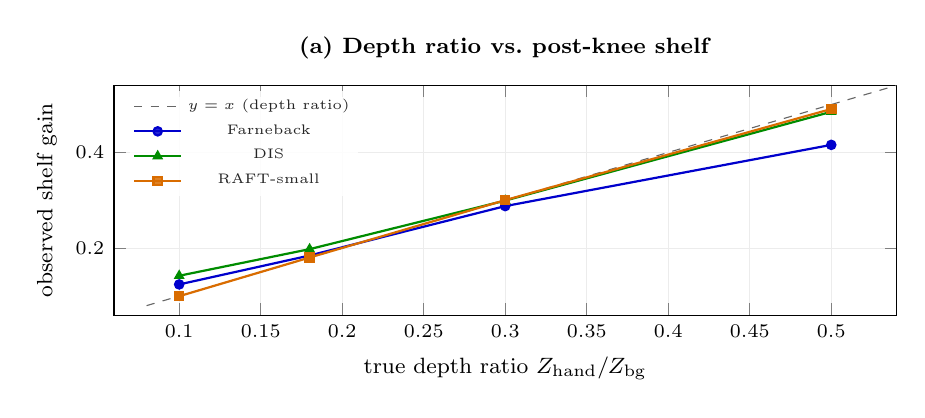
\begin{tikzpicture}
\begin{axis}[width=0.95\linewidth,height=4.5cm,title={\footnotesize\textbf{(a) Depth ratio vs.\ post-knee shelf}},xlabel={\footnotesize true depth ratio $Z_{\mathrm{hand}}/Z_{\mathrm{bg}}$},ylabel={\footnotesize observed shelf gain},xmin=0.06,xmax=0.54,ymin=0.06,ymax=0.54,legend style={at={(0.02,0.98)},anchor=north west,font=\tiny,draw=none,fill=white,fill opacity=0.85,inner sep=1pt},grid=both,grid style={gray!15},tick label style={font=\scriptsize}]
\addplot[black!60,dashed,thin] coordinates {(0.08,0.08)(0.54,0.54)};
\addlegendentry{$y=x$ (depth ratio)}
\addplot[blue!80!black,thick,mark=*,mark size=1.5pt] coordinates {(0.500,0.4158) (0.300,0.2879) (0.180,0.1847) (0.100,0.1243)};
\addlegendentry{Farneback}
\addplot[green!55!black,thick,mark=triangle*,mark size=1.5pt] coordinates {(0.500,0.4849) (0.300,0.2994) (0.180,0.1980) (0.100,0.1424)};
\addlegendentry{DIS}
\addplot[orange!85!black,thick,mark=square*,mark size=1.5pt] coordinates {(0.500,0.4907) (0.300,0.3004) (0.180,0.1805) (0.100,0.0997)};
\addlegendentry{RAFT-small}
\end{axis}
\end{tikzpicture}
\end{minipage}\hfill
\begin{minipage}{0.49\linewidth}
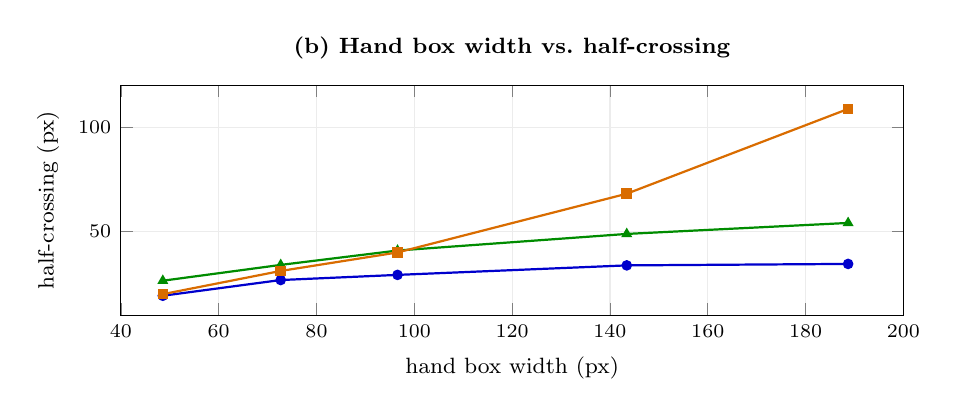
\begin{tikzpicture}
\begin{axis}[width=0.95\linewidth,height=4.5cm,title={\footnotesize\textbf{(b) Hand box width vs.\ half-crossing}},xlabel={\footnotesize hand box width (px)},ylabel={\footnotesize half-crossing (px)},xmin=40,xmax=200,ymin=10,ymax=120,grid=both,grid style={gray!15},tick label style={font=\scriptsize}]
\addplot[blue!80!black,thick,mark=*,mark size=1.5pt] coordinates {(48.569,19.3131) (72.672,26.8393) (96.561,29.3008) (143.431,33.8532) (188.697,34.5493)};
\addplot[green!55!black,thick,mark=triangle*,mark size=1.5pt] coordinates {(48.569,26.5167) (72.672,34.0845) (96.561,40.9645) (143.431,48.9097) (188.697,54.1700)};
\addplot[orange!85!black,thick,mark=square*,mark size=1.5pt] coordinates {(48.569,20.0737) (72.672,31.1868) (96.561,40.0428) (143.431,68.1538) (188.697,108.7450)};
\end{axis}
\end{tikzpicture}
\end{minipage}

\vspace{4pt}
\begin{minipage}{0.49\linewidth}
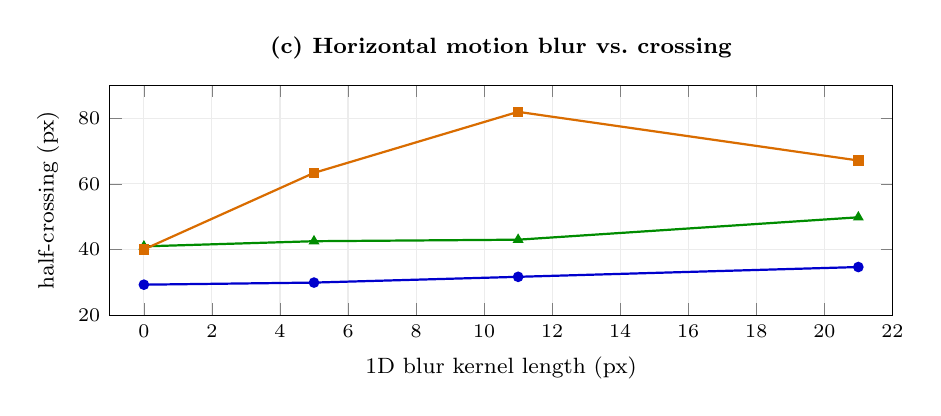
\begin{tikzpicture}
\begin{axis}[width=0.95\linewidth,height=4.5cm,title={\footnotesize\textbf{(c) Horizontal motion blur vs.\ crossing}},xlabel={\footnotesize 1D blur kernel length (px)},ylabel={\footnotesize half-crossing (px)},xmin=-1,xmax=22,ymin=20,ymax=90,grid=both,grid style={gray!15},tick label style={font=\scriptsize}]
\addplot[blue!80!black,thick,mark=*,mark size=1.5pt] coordinates {(0.000,29.3008) (5.000,29.9376) (11.000,31.6929) (21.000,34.6747)};
\addplot[green!55!black,thick,mark=triangle*,mark size=1.5pt] coordinates {(0.000,40.9645) (5.000,42.5415) (11.000,43.0026) (21.000,49.8260)};
\addplot[orange!85!black,thick,mark=square*,mark size=1.5pt] coordinates {(0.000,40.0428) (5.000,63.3612) (11.000,81.9475) (21.000,67.1272)};
\end{axis}
\end{tikzpicture}
\end{minipage}\hfill
\begin{minipage}{0.49\linewidth}
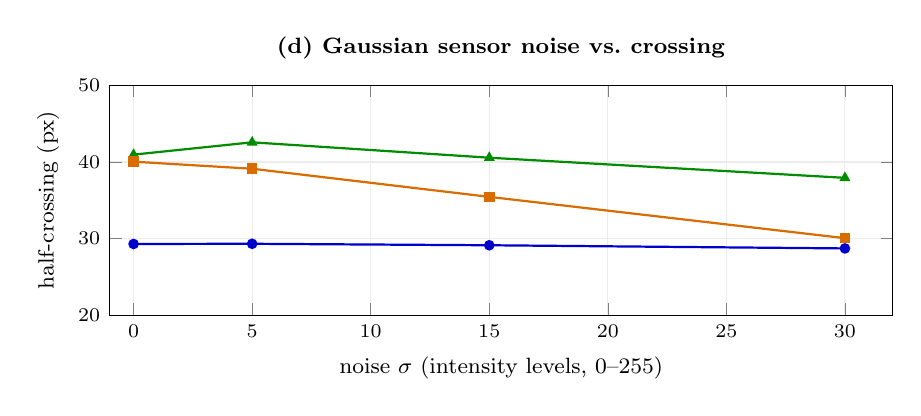
\begin{tikzpicture}
\begin{axis}[width=0.95\linewidth,height=4.5cm,title={\footnotesize\textbf{(d) Gaussian sensor noise vs.\ crossing}},xlabel={\footnotesize noise $\sigma$ (intensity levels, 0--255)},ylabel={\footnotesize half-crossing (px)},xmin=-1,xmax=32,ymin=20,ymax=50,grid=both,grid style={gray!15},tick label style={font=\scriptsize}]
\addplot[blue!80!black,thick,mark=*,mark size=1.5pt] coordinates {(0.000,29.3008) (5.000,29.3250) (15.000,29.1331) (30.000,28.7196)};
\addplot[green!55!black,thick,mark=triangle*,mark size=1.5pt] coordinates {(0.000,40.9645) (5.000,42.5713) (15.000,40.5631) (30.000,37.9339)};
\addplot[orange!85!black,thick,mark=square*,mark size=1.5pt] coordinates {(0.000,40.0428) (5.000,39.1236) (15.000,35.4506) (30.000,30.0584)};
\end{axis}
\end{tikzpicture}
\end{minipage}
